\begin{figure}[!t]
	\centering
	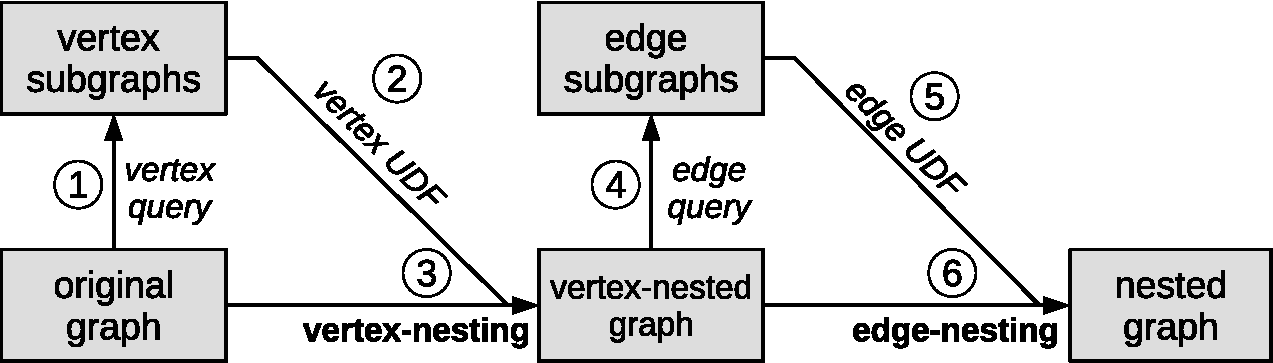
\includegraphics[width=0.8\textwidth]{fig/06nesting/overview.pdf}
	\caption{Overview about the general graph nesting process. UDF stands for \textsc{User Defined Function}.}
	\label{fig:process}
\end{figure}
\subsection{Implementing Graph Nesting over (two) graph collections}\label{subsec:polyovergraph}

In order to create nested vertices and edges, we can first propose a generic \textit{nesting operator}, allowing the creation of arbitrary vertices and edges over a given (nested) graph (\textbf{original} or \textbf{input graph}). Figure \ref{fig:process} provides an overview about the nesting process. First, in step \textcircled{\raisebox{-.5pt}1} a \textit{query} is used to determine subgraphs which will later on be nested as vertices' content. In Example \vref{ex:nestingbib}, we want to nest each \textsc{Author} with its egonet represented by the paper he has authored, and hence we're going to extract all the subgraphs matching the pattern $\textsc{Author}\overset{\texttt{authorOf}}{\longrightarrow}\textsc{Paper}^*$ (Figure \ref{fig:vertexPat}). Another example is the Social Network scenario presented in Example \vref{ex:8}: we want to nest each user of the \texttt{DataSource} in her or his \texttt{Community}. Here, the term \textit{query} generally refers to either a pattern matching query (e.g., a community can defined by each user's egonet) or a partitioning algorithm (e.g., community detection). As a consequence, the way to extract subgraphs to be summarized as vertices is application dependent, and may require a previous graph traversal phase or not.


%%  
%% This operation could be either expressed through 
%
Subsequently, in step \textcircled{\raisebox{-.5pt}2} a \textsc{User Defined Function} (UDF) can be applied to the resulting subgraphs in order to derive aggregated vertices from the subgraph's elements that will be added to the final nested vertex. In particular, in a data integration scenario one could select representative property values to appear in the resulting vertex or, in a summarization process, one could evaluate measures such as vertex count over the extracted graph. The subsequent step \textcircled{\raisebox{-.5pt}3} takes the original graph as well as the processed subgraphs as input and turns the latter into nested vertices. The resulting vertex-nested graph contains all the nested vertices from \textcircled{\raisebox{-.5pt}3}, containing at least one vertex also nested in the original graph, but also all vertices of the original graph not appearing in one of the subgraphs. In the Social Network scenario, the previous steps could have been performed by an external community detection algorithm. 

% These two conditions shall be expressed by a pattern matching language over the two filtered datasets, thus allowing to express the vertex and edge containment conditions. 
%%Referring to Figure \ref{fig:osn}, the input of the vertex-nesting operation is the \texttt{DataSource} nested vertex, the result of a community detection algorithm \texttt{GraphCollection}, and an empty UDF. The result is the nested vertex $10$ where only the vertices  $7$, $8$ and $3$ appear. The edges are then added in the subsequent phase.
%
In order to obtain the final nested graph from the vertex-nested graph, we must apply a similar process over the edges: in step \textcircled{\raisebox{-.5pt}4} subgraphs containing nested vertices can be extracted using a dedicated query. These subgraphs form the basis of the later nested edges where, using our running example, they can be previously extracted by visiting the pattern $\textsc{Author}\overset{\texttt{authorOf}}{\longrightarrow}\textsc{Paper}^*\overset{\texttt{authorOf}}{\longleftarrow} \textsc{Author}$ (Figure \ref{fig:pathPat}). In contrast to vertices, an UDF (step \textcircled{\raisebox{-.5pt}5}) is mandatory since its purpose is not only to aggregate properties but also to select source and target on the later nested edge of step \textcircled{\raisebox{-.5pt}6}. These can be both nested and simple vertices. For example, in a summarization scenario a nested edge may connect two previously nested vertices while in a transformation scenario it can replace a path between two simple vertices. Consequently, before adding edges between vertices that do not appear in the vertex-nested graph, we must also ensure that such UDF generate valid edges. Please note that, also in this case, phases \textcircled{\raisebox{-.5pt}4} and \textcircled{\raisebox{-.5pt}5} can be also carried out by an external algorithm.
%%Referring to Figure \ref{fig:osn}, the nested vertex $10$ represents the final outcome of this phase: edges $\Braket{7,8}_x$ and $\Braket{8,7}_{\textit{ix}}$ are created because \texttt{User} ``Evelyn'' from \texttt{Community} $7$ follows  \texttt{User} ``Basil'' from \texttt{Community} $8$, and vice versa. Moreover, edge $\Braket{8,3}_{\textit{viii}}$ is also created because \texttt{User} ``Basil'' from \texttt{Community}  $8$ follows \texttt{User} ``Carey'', which does belong to no \texttt{Community}.
%
%% This last UDF must be general enough to represent a pattern matching query: in particular, it should transform a nested vertex into one or more nested edges (possibly) with the same vertex and edge content. 
%% 
%% Each one of these edges $\Braket{i,j}_k$ has as a source $i$ which is either a nested vertex, sharing with $k$ either the vertex or the edge content (e.g., $\phi(i)\cap\phi(\Braket{i,j_k})\neq \emptyset \vee \omega(i)\cap\omega(\Braket{i,j_k})\neq \emptyset$), or a simple vertex, appearing in its nesting (e.g., $i\in \phi(\Braket{i,j}_k)$). Similar property must hold also for target vertices. 
%
%

\begin{algorithm}[!t]
	\caption{General Nesting Algorithm}\label{alg:generalNesting}
	\begin{adjustbox}{max width=\textwidth}
		\begin{minipage}{1.2\linewidth}
			\begin{algorithmic}[1]
				\Procedure{GeneralNesting}{$(\mathcal{G}_V,\texttt{UDF}_V),(\mathcal{G}_E,\texttt{UDF}_E),\textbf{keep} ;\;\nested$}
				\State{$GV=\emptyset;\quad GE=\emptyset;\quad VR=\emptyset;\quad ER=\emptyset$}
				\For{\textbf{each graph }$g_v=(V,E)$ in $\mathcal{G}_V$}
					\State{$\delta V = V\cap\phi(\ngraph,\ONTA)$}
					\State{$\delta E = E\cap\phi(\ngraph,\RELA)$}
					\If{$\delta V\neq \emptyset \vee \delta E\neq \emptyset$}
					\State $GV=GV\cup\{UDF_V(g_v)\}$
					\If{\textbf{keep}}
						\State{$VR=VR\cup \phi(\ngraph,\ONTA)\backslash \delta V$}
						\State{$ER=ER\cup \phi(\ngraph,\RELA)\backslash \delta E$}
					\EndIf
					\EndIf
				\EndFor	
				\For{\textbf{each graph }$g_e=(V,E)$ in $\mathcal{G}_E$}
				\State{$\delta V = V\cap\phi(\ngraph,\ONTA)$}
				\State{$\delta E = E\cap\phi(\ngraph,\RELA)$}
				\If{$\delta V\neq \emptyset \vee \delta E\neq \emptyset$}
				\State{$\varepsilon=UDF_E(g_e)$}
				\If{$\lambda(\varepsilon)\in (GV\cup \phi(\ngraph,\ONTA))^2 $}
				\State {$GE=GE\cup\{\varepsilon\}$}
				\If{\textbf{keep}}
					\State{$VR=VR\cup \phi(\ngraph,\ONTA)\backslash \delta V$}
					\State{$ER=ER\cup \phi(\ngraph,\RELA)\backslash \delta E$}
				\EndIf
				\EndIf
				\EndIf
				\EndFor	
				\State \Return $(GV\cup VR,GE\cup ER)$
				\EndProcedure
				
			\end{algorithmic}
		\end{minipage}
	\end{adjustbox}
\end{algorithm}

The unfeasibility of this naïve approach is remarked by Algorithm \vref{alg:generalNesting}: given that any to-be-nested graph may come from an external source, it is required that each graph collection pertaining either to the to-be-nested vertices (\textcircled{\raisebox{-.5pt}1}-\textcircled{\raisebox{-.5pt}3})  or edges (\textcircled{\raisebox{-.5pt}4}-\textcircled{\raisebox{-.5pt}6}) must be  analysed in order to get which elements are matched within the vertices and edges of the nested graph $\nested$. Only after this second visiting process, we can then apply the UDF function over the filtered graphs. This means that we must at least visit $\nested$ after each collection, with a cost of $|\nested|^{|\mathcal{G}_V|}+|\nested|^{|\mathcal{G}_E|}$, where ${|\mathcal{G}_V|}$ and ${|\mathcal{G}_E|}$ are the graph collections generated respectively from the vertex and the edge subgraph extraction process. The expensiveness of such approach is going to be later on compared to a more efficient algorithm for a specific subproblem (THoSP, Section \ref{sec:THOSPA}). This cost must be further on increased if we want to preserve the un-matched vertices and edges in the final graph (\textbf{keep}=\textbf{true}). Therefore, we want to decrease this computational post whenever possible: given that nesting is a specific case of summarization\footnote{Compare this statement with the formal definitions of semistructured and relational nesting proposed in Definition \vref{def:semistructnest}.}, we can observe that the previously proposed graph summarization algorithms provide one possible algorithmic enhancement for the cases when the graph is represented by an exact partition, as when we group the graph by either its labels or attributes \cite{JunghannsPR17}. As previously observed, the purpose of this chapter is instead to extend the family of such graph nesting algorithms by combining pattern matching approaches to the nesting process: instead of generating multiple graph collections with an external method for then nesting them, we want to compactly generate them while visiting the graph. Then, the visited graph will be immediately used to generate a nesting, thus combinating the graph visit process with the nesting one, thus allowing to decrease the overall time complexity. We're going to tackle this problem in Section \vref{sec:optimizableClass} after providing a formal definition of such operator in Section \vref{sec:nestingdef}.


\subsection{Query Languages' and data models' limitations}\label{subsec:pathsumm}
As previously mentioned, some recent  query languages support graph nesting semantics by exploiting the underlying data model's features. To express the query presented in our running example, these query languages must support id collections or nested representations.
For these reasons, we firstly select PostgreSQL which, by extending the SQL-3 syntax and by allowing JSON data, provides an \texttt{array\_agg} aggregation function. The latter collects (i.e., groups) the result-set into arrays.  We  represent  graphs by  storing edge triples as \texttt{Edge}(\textit{edgeId},\;\textit{sourceId},\;\textit{edgeLabel},\;\textit{targetId}).
In our running example, nested vertices  are obtained by 
grouping edges by \textit{sourceId} and collecting all target's id results via \texttt{array\_agg}. Similarly, our nested edges are obtained by joining consecutive \texttt{Edge}s and then grouping  by  distinct \textit{sourceId} and \textit{targetId}  vertices limiting the two hop path; the list of all the \textsc{Paper}s is collected via \texttt{array\_agg}. The overall graph nesting cannot be created in one single SQL query, because we cannot distinctively group the same dataset in different ways. Instead, we must perform two distinct aggregations (see Listing \ref{SQLNesting}).
We want now to discuss how current query languages can express nesting constraints within their data model of choice. In particular, we must select query languages that either support collections or nested representations allowing to express the same query presented in our running example. 

%For these reasons, we select PostgreSQL's dialect which, by extending the SQL-3 syntax with JSON data supports, allows to create array as a result of a \texttt{GROUP BY} query via \texttt{array\_agg}; therefore, instead of using function aggregating a collection into one single summarized value, we can list all the elements that have been aggregated. In particular, in PostgreSQL's dialect, we choose implement our graph by only storing the triples defining an \texttt{Edge}(\textit{edgeId},\;\textit{sourceId},\;\textit{edgeLabel},\;\textit{targetId}) relation: hereby, by grouping the edges by \textit{sourceId} and collecting all the target's ids we obtain a representation of nested vertices. Similarly, if we join the \texttt{Edge} relation with itself and group the join result by two distinct \textit{sourceId} and return the list of all the \textsc{Paper}s that they have in common, we can return the list of all the \textsc{Paper}s that they have coauthored. As showed in Listing \ref{SQLNesting}, the overall graph nesting cannot be created in one single SQL query, because by  the SQL language definition we cannot distinctively group the same dataset in different ways, but we must visit the same data twice and perform two distinct aggregations. 

\begin{lstfloat}
\begin{lstlisting}[caption={Graph Nesting in PostgreSQL. Two distinct tables are created for both vertices and edges. The nesting is represented by nesting the elements' id within an array (\texttt{array\_agg}). Please note that such sybtax is not SQL-3 standard.},language=SQL,frameround=fttt,frame=trBL,mathescape=true,label=SQLNesting]
-- Nesting Vertices
SELECT distinct T.sourceId as src, array_agg(distinct T.dst) as papers 
FROM edges-$i$ as T 
GROUP BY T.sourceId;

-- Nesting Edges
SELECT distinct T.sourceId as src, T1.sourceId as dst, 
       array_agg(distinct T1.targetId) as papers
FROM edges-$i$ as T, edges-$i$ as T1 
WHERE T.targetId = T1.targetId AND T.sourceId <> T1.sourceId 
GROUP BY T.sourceId, T1.sourceId;
\end{lstlisting}

\begin{lstlisting}[caption={Graph Nesting in SPARQL. Given that the RDF List solution is inefficient and that named graphs cannot be used either in the RDF models as vertices or edges, we use other properties to associate to either vertices and edges the nesting content.},language=SPARQL,frameround=fttt,frame=trBL,tabsize=2,mathescape=true,label=SPARQLNesting]
CONSTRUCT {
	?autha ?newedge ?authb.
	?newedge <http://contains.io/nesting> ?paper1.
	?authc <http://test.graph/graph/edge> ?paper2.
} WHERE {
	{
		GRAPH <http://test.graph/graph/$i$/> {
			?autha <http://test.graph/graph/edge> ?paper1.
			?authb <http://test.graph/graph/edge> ?paper1.
		}
		FILTER(?autha != ?authb).
		BIND(URI(CONCAT("http://test.graph/graph/newedge/",STRAFTER(STR(?autha),"http://test.graph/graph/id/"),"-",STRAFTER(STR(?authb),"http://test.graph/graph/id/"))) AS  ?newedge).
	} UNION {
		GRAPH <http://test.graph/graph/$i$/> {
			?authc <http://test.graph/graph/edge> ?paper2.
		}
		OPTIONAL {
			?authd <http://test.graph/graph/edge> ?paper2.
			FILTER (?authd != ?authc)
		}
		FILTER(!bound(?authd))
	}
}
\end{lstlisting}
\end{lstfloat}


\begin{lstfloat}[!p]
\begin{lstlisting}[caption={Graph Nesting in ArangoDB using AQL as a query lanugage. Please note that all the fields marked with an underscore represent externally indexed structures and. Therefore, only external indices are used within the query plan.},language=AQL,frameround=fttt,frame=trBL,tabsize=2,mathescape=true,label=AQLQueryNesting]
-- Nesting vertices
FOR b IN authorOf 
	COLLECT au = b._from INTO groups = [ b._to ] 
	RETURN {"author" : au,  "papers": groups }
	
-- Nesting edges
FOR x IN authorOf 
	FOR y IN authorOf 
		FILTER x._to == y._to && x._from != y._from 
		COLLECT src = x._from, dst = y._from INTO groups = [ x._to ] 
		RETURN {"src": src, "dst": dst, "contain": groups}
\end{lstlisting}
	
\begin{lstlisting}[caption={Graph Nesting in Neo4J using Cypher as a Query Language. Please note that, even in this case, is it not possible to return one single nested graph immediately, and hence the nested vertices must be created before creating the nested edges. This implies that a greater number of joins is required to associate the previously nested data to the original operand.},language=Cypher,frameround=fttt,frame=trBL,mathescape=true,label=Neo4JQuery]
MATCH (a1: Author)-->(p1:Paper) 
WITH a1, collect(p1.UID) AS papers1 
CREATE  p=(:Authors {authored: papers1, id:a1.UID})
	
MATCH (a1: Author)-->(p:Paper)<--(a2: Author), (a1p: Authors), (a2p: Authors)
WITH a1, a2, a1p, a2p, collect(p.UID) AS common
WHERE a1.UID = a1p.id AND a2.UID = a2p.id AND a1.UID <> a2.UID
CREATE p=(a1p)-[:Papers {coauthored: common}]->(a2p)
\end{lstlisting}
\end{lstfloat}


All the other query languages are going to be affected by the same problem, SPARQL included (Listing \ref{SPARQLNesting}): despite the fact that SPARQL  may represent the graph nesting query as a single statement, a \texttt{UNION} clause implies a separate visit for the two graph patterns. The first pattern presented in Listing \ref{SPARQLNesting} (see Appendix) allows to traverse those  patterns matching the coauthorship statement in Figure \ref{fig:pathPat}, so that they can be nested within the created \textsc{CoAuthorship} edge. The second part returns the remaining \textsc{Paper} associations that have been authored by one single \textsc{Author}. In the first case, the edge nesting is performed via the association of different \texttt{<http://contains.io/nesting>} properties departing from one single  \textsc{coAuthorship} edge (\texttt{?newedge}). In particular, the \texttt{OPTIONAL\dots FILTER(!bound(\dots))} syntax is adopted instead of \texttt{FILTER NOT EXISTS}, because the latter is only supported in SPARQL1.1, which is not supported by the current version of \textit{librdf} used to query Virtuoso.

We extend our query languages comparison presented on graph joins (Chapter \ref{cha:join}) with AQL, because ArangoDB is a document-oriented NoSQL database, which query language AQL allows the access and the creation of nested members. An example of how such graph nesting query can be carried out in AQL is presented in Listing \ref{AQLQueryNesting}: in this scenario we assume that we've previously loaded our graph data with the default ArangoDB format, where  vertices are indexed by id while edges are also indexed by source and target vertex id\footnote{\url{https://docs.arangodb.com/3.2/Manual/Graphs/}}. Even though AQL returns JSON documents instead of relational tables, we can state that its resulting query plan is similar to PostgreSQL's query plan, except that JSON documents are returned instead of relational tables containing JSON arrays.
%
%Let us consider the following query that will be express in our different languages:
%``\textit{Total number of orders handled by each employee. Only list employees that handled more than 100 orders}''
%
%At this point we immediately notice that NautiLOD and G could not express the summarization since those languages
%are graph traversal languages for pattern matching: consequently they could only select paths and subgraphs but
%they do not aggregate (summarize) nodes. In this case a bag of both employees and the number of the orders
%is returned. Since the result is a bag of values, we cannot obtain a graph as an output, and hence we cannot establish some new edges through the employee and the aggregated value of the sales.
%
%\begin{lstlisting}[caption={Summarization query in Gremlin},language=gremlin,frameround=fttt,frame=trBL]
%graph = TinkerGraph.open()
%graph.io(IoCore.gryo()).readGraph('/path/to/graph')
%g = graph.traversal()
%
%g.V().hasLabel("Employee").match(
%      __.as("emp").in("SalesEmployee").hasLabel("Sales").count()
%                                      .as("ordersByEmployee"),
%      __.as("ordersByEmployee").is(gt(100))
%).select("emp", "ordersByEmployee")
%\end{lstlisting}
%\medskip
%
%The SPARQL query returns a table with two attributes, where the first is the Employee ID and the
%second element is the number of its handled orders. In this case the output is expressed as a table.
%
%\begin{lstlisting}[caption={Summarization query in SPARQL: Table},language=sparql,frameround=fttt,frame=trBL]
%PREFIX ex:<http://example.it/Relations#>
%
%SELECT	 ?emp, (COUNT (?sales) AS ?ordersByEmployee)
%WHERE    {
%          ?sales a                 ex:Sales;
%                 ex:SalesEmployee  ?emp.
%          ?emp   a                 ex:Employee.    
%         }
%GROUP BY ?emp
%HAVING   COUNT(?orderNo) > 100
%\end{lstlisting}
%
%With the \texttt{\textbf{CONSTRUCT}} clause we could return the previous result inside an RDF Graph.
%\begin{lstlisting}[caption={Summarization query in SPARQL: Graph},language=sparql,frameround=fttt,frame=trBL]
%PREFIX ex:<http://example.it/Relations#>
%
%CONSTRUCT { ?ordersByEmployee ex:SalesEmployee ?emp. }
%WHERE {{
%	SELECT	 ?emp, (COUNT (?sales) AS ?ordersByEmployee)
%	WHERE    {
%	          ?sales a                 ex:Sales;
%	                 ex:SalesEmployee  ?emp.
%	          ?emp   a                 ex:Employee.    
%	}
%	GROUP BY ?emp
%	HAVING   COUNT(?orderNo) > 100
%}}
%\end{lstlisting}
%\medskip
%
%In Cypher we could formulate a similar query with a tabular result as follows:
%\begin{lstlisting}[caption={Summarization query in Cypher: Table},language=cypher,frameround=fttt,frame=trBL]
%MATCH  (sales:Sales)-[:SalesEmployee]->(empl:Employee)
%WITH   empl AS emp, COUNT(sales) AS ordersByEmployee
%WHERE  ordersByEmployee > 100
%RETURN empl, ordersByEmployee
%\end{lstlisting}
%
%With this language we could even return a new graph, where
%the whole information of the employee is returned and where the films are aggregated.
%\begin{lstlisting}[caption={Summarization query in Cypher: Graph},language=cypher,frameround=fttt,frame=trBL]
%MATCH  (sales:Sales)-[:SalesEmployee]->(empl:Employee)
%WITH   empl AS emp, COUNT(sales) AS ordersByEmployee
%WHERE  ordersByEmployee > 100
%CREATE p=
%(:Sales {count: ordersByEmployee})-[:SalesEmployee]->(empl:Employee)
%RETURN p
%\end{lstlisting}
%\medskip 
%
%Let us now focus on the BiQL language: firstly we cannot create new vertices that aggregate the results without
%updating the original database because the \texttt{\textbf{CREATE}} semantic has this precise meaning, secondly the
%\texttt{\textbf{CREATE}} clause does not allow to create multiple objects within the same query: this means that we 
%cannot create new edges while creating new vertices. By the way we could return all the employees and store the
%number of the sales inside each node.
%\begin{lstlisting}[caption={Summarization query in Cypher: Graph},language=biql,frameround=fttt,frame=trBL]
%SELECT <empl>{empl.*, ordersByEmployee: count(salesEdge)}
%FROM   Employee empl <- SalesEmployee salesEdge 
%WHERE  count(salesEdge) > 100
%\end{lstlisting}
%

Last, Listing \ref{Neo4JQuery} provides an example of Cypher: even if Neo4J's property graph model does not directly nest graphs inside vertices or edges, we can associate \textit{member} ids to each of them. This solution can be achieved by  first matching the vertex summarization pattern of Figure \ref{fig:vertexPat} and then performing an \textsc{Author} group by (\texttt{with}). Afterwards, we nest the set of authored \textsc{Paper}s via \texttt{collect}. Last, we match the path summarization pattern presented in Figure \ref{fig:pathPat} and group it by source and destination \textsc{Author}, then we create the \textsc{coAuthorship} edge containing the co-authored \textsc{Paper}'s id. As it will be observed within the benchmarks (see Section \ref{sec:nestexpeval}), the solution of not separating the elements' ids from their data quickly leads to an intractable solution.

In all the former query languages, the vertices undergoing  \texttt{GROUP BY}-s are either vertex or edge grouping references.

%Last, Listing \vref{Neo4JQuery} provides an example of Neo4J allowing to nest property graphs: even in this case the property graph model does not directly  nest the graphs inside one element. Similar to the previous approaches, we can group by all the graphs returned by the graph pattern by selecting the vertices of interest, and nesting the to-be-grouped remaining objects inside a collection. In particular, we can first match the vertex summarization pattern in Figure \vref{fig:vertexPat} and group by \textsc{Author}, and nest the collection of authored \textsc{Paper}s within the to-be-created nested vertex; similarly, we can first match the path summarization pattern presented in Figure \ref{fig:pathPat} by source and destination \textsc{Author}, and then create an edge between the previously created nested vertices by collecting all the coauthored \textsc{Paper}s appearing in the original graph. Moreover, the Neo4J property graph data model forces us not to create an edge if the vertices are not already known. As a consequence, we always must join the nested vertices with the original matched ones in order to reconstruct the original information and perform the actual matching operation. As it will be observed within the benchmarks (see Section \ref{sec:nestexpeval}), the solution of not separating the elements' ids from their data quickly leads to an intractable solution.

